\subsubsection{Perfectly Matched Layer Method} \label{PerfectlyMatchedLayerMethodSection}

The Perfectly Matched layer technique is fundamentally very simple, whereby a complex change of variable is applied on the spatial variable within the frequency domain \cite{parrish2008analysis}. That is to say, the derivation follows 3 steps: 1. a space-time transformation to ensure cohesive group/phase velocities, 2. a complex change of variables (in the frequency domain) to introduce absorption coefficients, and 3. reverse space-time transformation and restoration of the time dependence. Early derivations \cite{hu1996onabsorbingbc} \cite{parrish2008analysis} sought to split the formulation into $x-$, $y-$, and corner layer sets-of-equations. This practice was then streamlined to unsplit formulations \cite{hu2001astablePML} \cite{tam2012computational} which are relatively easier to implement computationally (see Section \ref{NumMethSect}) due to the PML equations being standardised across the domain. Additionally, split PML formulations are found to be weakly well-posed \cite{abarbanel1997mathanalysispml}, and the unsplit formulations are shown to eliminate undesirable long-term linear growth (via the similar electromagnetic formulation) \cite{becache2004longtime}. Figure \ref{fig:PMLDomain} illustrates the domain with absorbing zone PMLs.

\begin{figure}[h!]
\centering
\makebox[0pt]{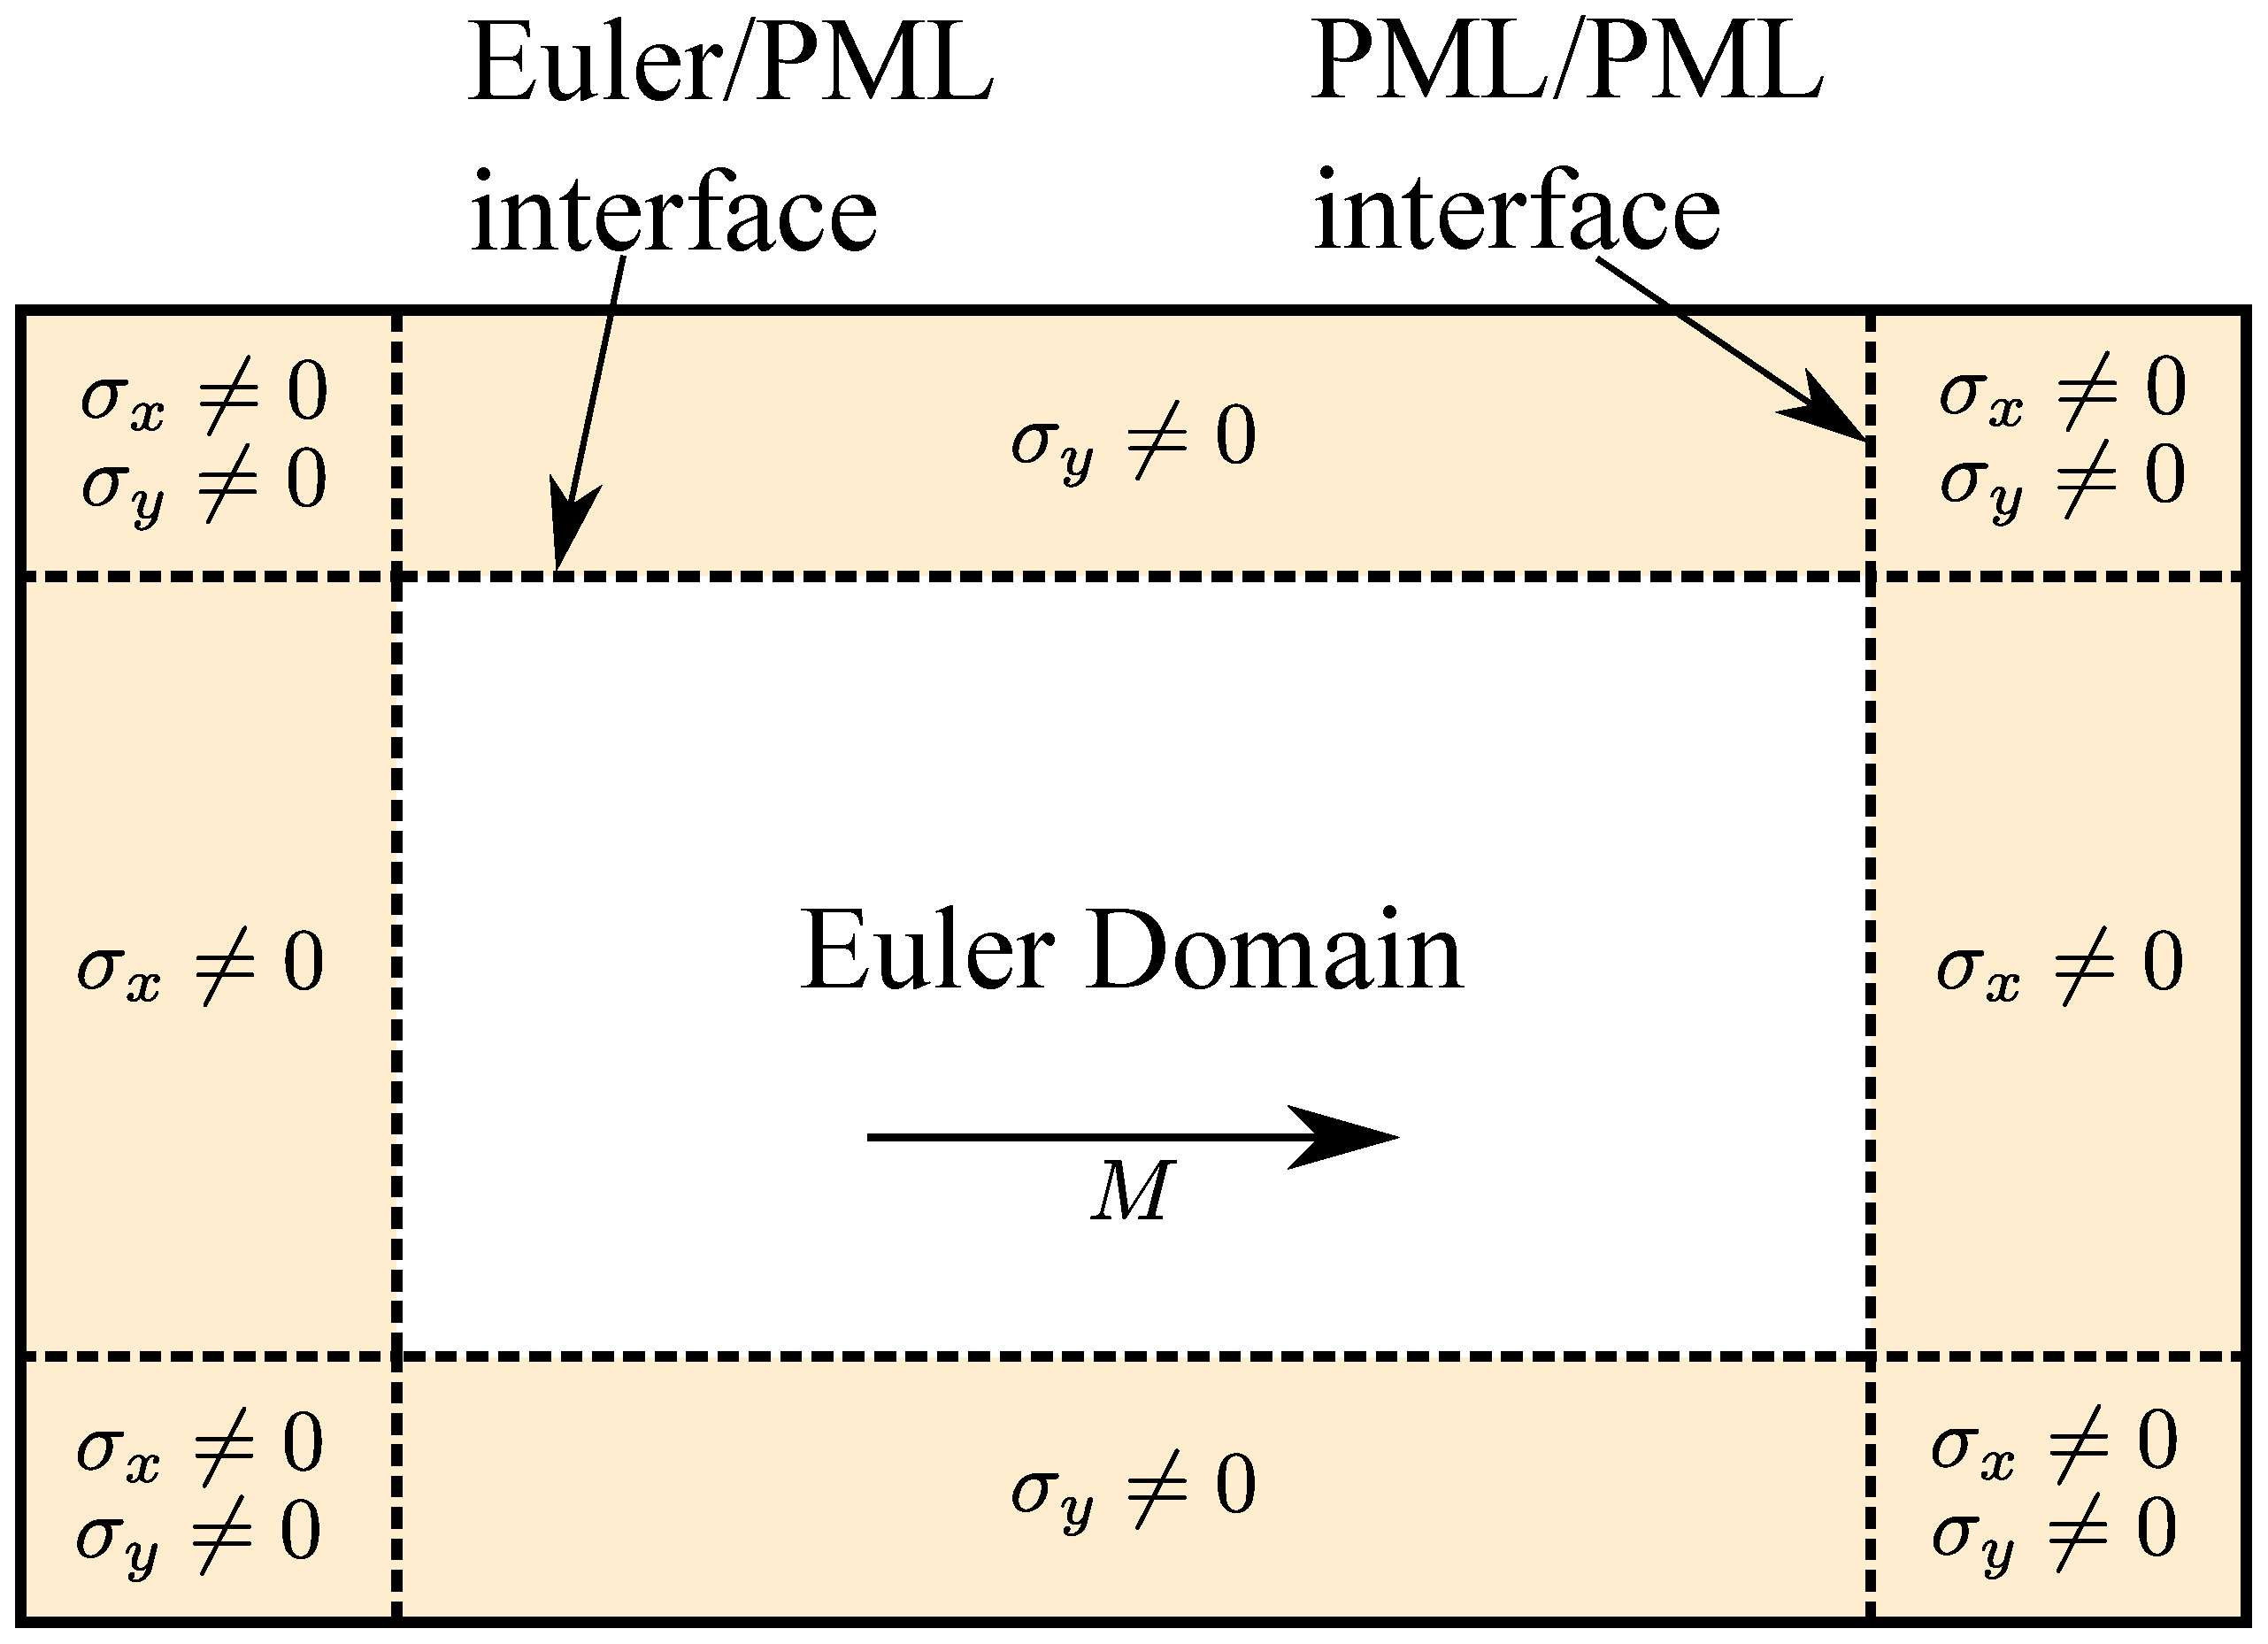
\includegraphics[width=9cm]{Figures/TechnicalAchievement/PMLBC/PMLDomain.eps}}
\caption{Computational domain highlighting boundary zones (layers) of non-zero damping and one-directional mean flow.}
\label{fig:PMLDomain}
\end{figure}

For the purposes of the PML derivation, it is beneficial to rearrange Equation \ref{eq:LEE} from Section \ref{GovEqSection} to enforce a single operand $\mathbf{U}$ - operated on spatially and temporally. The dimensionless linearised Euler equation can thus be rewritten as

\begin{equation} \label{eq:DimensionlessEuler}
    \frac{\partial \mathbf{U}}{\partial t} + \mathbf{A}\frac{\partial \mathbf{U}}{\partial x} + \mathbf{B}\frac{\partial \mathbf{U}}{\partial y} = 0
\end{equation}
where
\begin{displaymath}
\mathbf{U} = 
\begin{bmatrix}
\rho \\
u \\
v \\
p
\end{bmatrix}, 
\mathbf{A} = 
\begin{bmatrix}
M & 1 & 0 & 0\\
0 & M & 0 & 1 \\
0 & 0 & M & 0 \\
0 & 1 & 0 & M
\end{bmatrix}, 
\mathbf{B} = 
\begin{bmatrix}
0 & 0 & 1 & 0\\
0 & 0 & 0 & 0 \\
0 & 0 & 0 & 1 \\
0 & 0 & 1 & 0
\end{bmatrix}
\end{displaymath}
Note the prime $\left( \ ' \right)$ has been dropped from the perturbation quantities.




As will be clarified \& reasoned in Section \ref{DispRelaStabSection}, the variables $(x,y,t)$ are first transformed in space-time to $(\Bar{x},\Bar{y},\Bar{t})$ (step 1)

\begin{equation} \label{eq:SpaceTimeTr}
\Bar{x} = x, \quad \Bar{y} = \gamma y, \quad \Bar{t} = t + \beta x \footnote[1]{incidentally this resembles the Prandtl-Glauert correction}
\end{equation}
where
\begin{displaymath}
\gamma = \sqrt{1-M^2}, \quad \beta = \frac{M}{\gamma^2}
\end{displaymath}


The transformed variables are then substituted back into the partial derivatives in Equation \ref{eq:DimensionlessEuler}

\begin{equation} \label{eq:TransformedLEE}
    \left( \mathbb{I} + \frac{M}{1-M^2} \mathbf{A} \right) \frac{\partial \mathbf{U}}{\partial \Bar{t}} + \mathbf{A} \frac{\partial \mathbf{U}}{\partial \Bar{x}} + \sqrt{\left(1-M^2\right)} \mathbf{B} \frac{\partial \mathbf{U}}{\partial \Bar{y}} = 0
\end{equation}

Equation \ref{eq:TransformedLEE} is time dependent such that a Fourier transform yields $\mathbf{U}\left(x,y,t\right)=\hat{\mathbf{U}}\left(x,y\right)e^{-\mathrm{i} \Bar{\omega}\Bar{t}}$. When substituted into the partial derivative WRT $\Bar{t}$, the term becomes $\frac{\partial \mathbf{U}}{\partial \Bar{t}}=- \mathrm{i} \Bar{\omega} \hat{\mathbf{U}}$. The remainder of Equation \ref{eq:TransformedLEE} is similarly Fourier transformed as


\begin{equation} \label{eq:FourierLEE}
    -\mathrm{i} \Bar{\omega} \left( \mathbb{I} + \frac{M}{1-M^2} \mathbf{A} \right) \hat{\mathbf{U}} + \mathbf{A} \frac{\partial \hat{\mathbf{U}}}{\partial \Bar{x}} + \sqrt{\left(1-M^2\right)} \mathbf{B} \frac{\partial \hat{\mathbf{U}}}{\partial \Bar{y}} = 0
\end{equation}

where $\left(\ \hat{} \ \right)$ denotes Fourier transformed quantities and $\mathbb{I}$ is an identity matrix.


The spatial variables undergo a complex change of variable so that the wave solution in the PML region decays exponentially with damping coefficient $\sigma$

\begin{equation} \label{eq:ComplexChange}
    x \rightarrow x + \frac{\mathrm{i}}{\Bar{\omega}} \int^{\Bar{x}}_{\Bar{x}_0} \sigma_{x} \left( x \right) \ dx , \quad y \rightarrow y + \frac{\mathrm{i}}{\Bar{\omega}} \int^{\Bar{y}}_{\Bar{y}_0} \sigma_{y} \left( y \right) \ dy
\end{equation}

which can be extended to the spatial derivatives \footnote[2]{note the $\sigma$ (damping coefficient) term is divided by $\omega$ (angular frequency) to ensure the shorter wavelengths decay at the same rate as longer wavelengths - as thoroughly described in \cite{johnson2021notesonPML}}

\begin{equation}
    \frac{\partial}{\partial \Bar{x}} \rightarrow \frac{1}{1 + \frac{\mathrm{i} \sigma_x \left( x \right)}{\Bar{\omega}}} \frac{\partial}{\partial \Bar{x}}, \quad \frac{\partial}{\partial \Bar{y}} \rightarrow \frac{1}{1 + \frac{\mathrm{i} \sigma_y \left( y \right)}{\Bar{\omega}}} \frac{\partial}{\partial \Bar{y}}
\end{equation}



These derivatives are then passed back into Equation \ref{eq:FourierLEE} (Step 2) to give

\begin{equation} \label{eq:ComplexFourierLEE}
    -\mathrm{i} \Bar{\omega} \left( \mathbb{I} + \frac{M}{1-M^2} \mathbf{A} \right) \hat{\mathbf{U}} + \frac{1}{1 + \frac{\mathrm{i} \sigma_x \left( x \right)}{\Bar{\omega}}} \mathbf{A} \frac{\partial \hat{\mathbf{U}}}{\partial \Bar{x}} + \frac{\sqrt{\left(1-M^2\right)}}{1 + \frac{\mathrm{i} \sigma_y \left( y \right)}{\Bar{\omega}}} \mathbf{B} \frac{\partial \hat{\mathbf{U}}}{\partial \Bar{y}} = 0
\end{equation}

The equation can now be reversed back to the original variables and have the time dependency restored (step 3). To do so, Equation \ref{eq:ComplexFourierLEE} is multiplied by $\left[1+\left(\mathrm{i}\sigma_x / \Bar{\omega} \right) \right]\left[1+\left(\mathrm{i}\sigma_y / \Bar{\omega} \right) \right]$, and an auxiliary term is introduced as $\hat{\mathbf{q}}= \hat{\mathbf{U}} \ \mathrm{i} / \Bar{\omega}$. The terms are then reverse-Fourier transformed and reverse-space-time transformed to yield Equation \ref{eq:FinalPML}. The inbetween steps of which are long and trivial, but a similar derivation can be found on p.160 of \cite{tam2012computational}.


\begin{equation} \label{eq:FinalPML}
\begin{split}
    \frac{\partial \mathbf{U}}{\partial t} + \mathbf{A} \frac{\partial \mathbf{U}}{\partial x} + \mathbf{B} \frac{\partial \mathbf{U}}{\partial y} + \left( \sigma_{x} + \sigma_{y} \right) \mathbf{U} + \sigma_{y} \mathbf{A} \frac{\partial \mathbf{q}}{\partial x} + \sigma_{x} \mathbf{B} \frac{\partial \mathbf{q}}{\partial y} \\
    + \sigma_{x}\sigma_{y}\mathbf{q} + \sigma_{x}\frac{M}{1-M^2} \mathbf{A}\left( \mathbf{U} + \sigma_{y} \mathbf{q} \right) = 0
    \end{split}
\end{equation}

where

\begin{equation} \label{eq:FinalPMLAux}
    \frac{\partial \mathbf{q}}{\partial t} = \mathbf{U}
\end{equation}

Note that when $\sigma_x = \sigma_y = 0$, Equation \ref{eq:FinalPML} degenerates into the linearised Euler equations (Equation \ref{eq:DimensionlessEuler}), thus attributing to the 'Perfectly Matched' descriptor\footnote[1]{the descriptor also refers to the PML mathematically avoiding reflections at the PML/Euler interface}. Effectively, the PML methods seeks to add a dissipative term to the main equations after they have been split along all spatial directions.

Naturally, the $\sigma_x$ and $\sigma_y$ damping coefficients are distributed across the PML zones, and require specification for doing so to ensure zero damping in the Euler domain - defined as

\begin{equation} \label{PMLProfileEq}
\sigma_{x} = \sigma_{\mathrm{max}_x} \Gamma \left( x \right) = \sigma_{\mathrm{max}_x} \left| \frac{x-x_0}{D_x} \right|^n
\end{equation}

where $\sigma_x$ is specified as the damping coefficient distribution across the domain's $x-$layers, $\sigma_{\mathrm{max}_x}$ is a set constant value, $\Gamma \left(x \right)$ is the absorption profile as a function of position $\left( x \right)$ in the domain, $D_x$ is the PML width, and $n$ is a positive real value providing a power-law. Note Equation \ref{PMLProfileEq} is also employed for the $y-$layer. 
The absorption profile should be such that at the location of the Euler/PML interface, $\sigma_{x} \left( x_0 \right) = \frac{\mathrm{d}\sigma_{x} \left( x_0 \right)}{\mathrm{d}x} = 0$ so that the Euler-PML interface is matched \cite{choung2018nonreflective}. For brevity, the maximum damping coefficient in the $x-$layer, $\sigma_{\mathrm{max}_x}$, will hereby be referred to as $\sigma_x$ - and so on with the $y-$layer. An illustration of the PML parameters can be seen below in Figure \ref{fig:PMLParameters}.

\begin{figure}[h!]
\centering
\makebox[0pt]{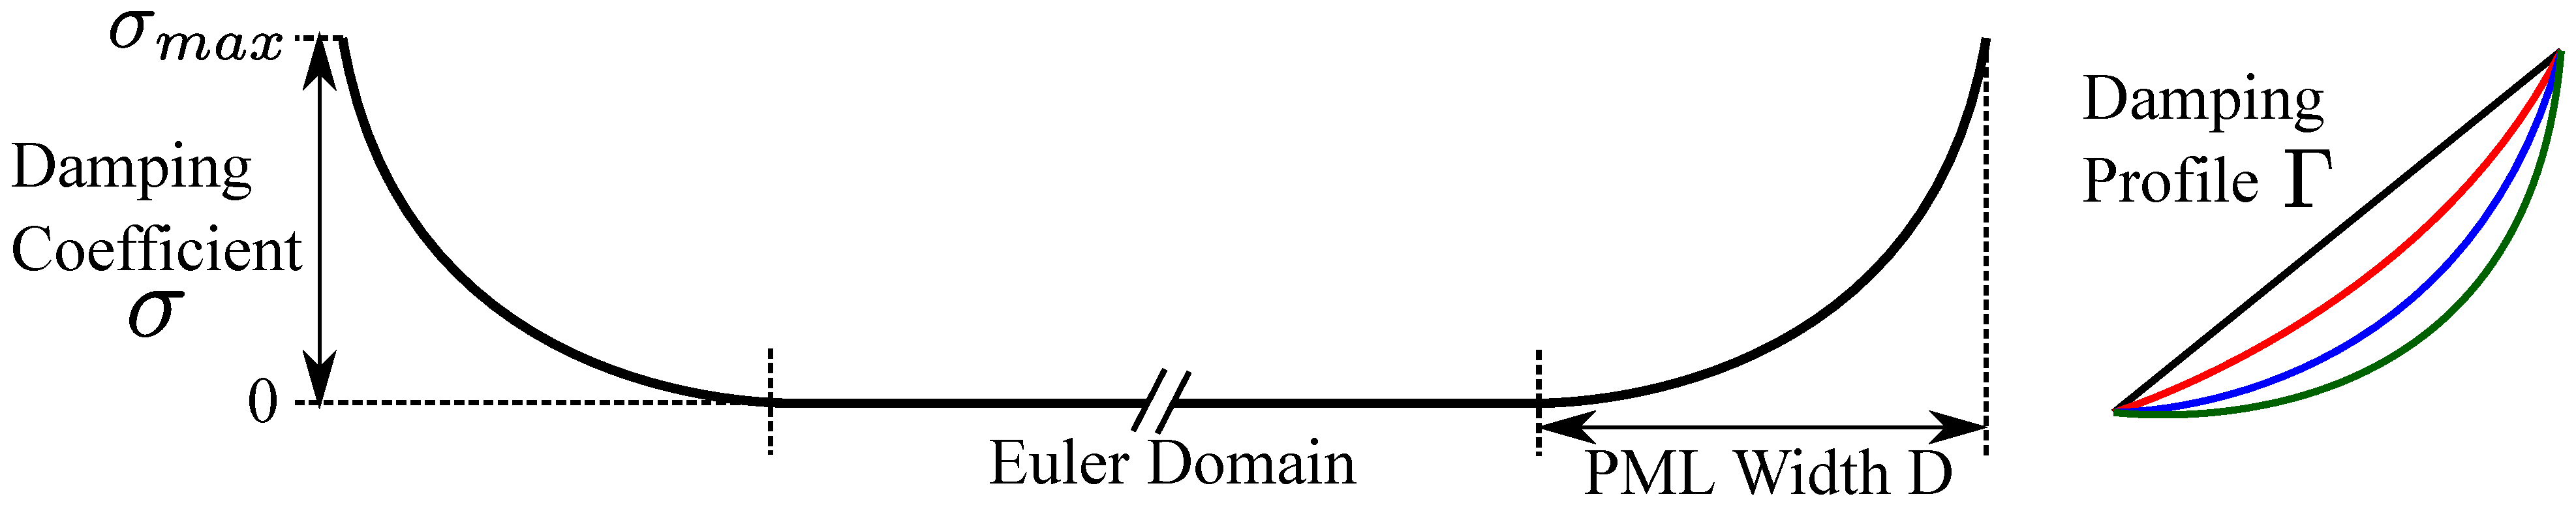
\includegraphics[width=14cm]{Figures/TechnicalAchievement/PMLBC/PMLParametersDia.eps}}
\caption{Illustrated PML Parameters: Damping coefficient, PML width, and Damping profile.}
\label{fig:PMLParameters}
\end{figure}
